\section{Analysis}
Our two basic research questions were addressed individually.

\subsection{Question 1}
To answer the first research question, we can rely on subjects' accuracy in distinguishing the two groups. We calculated this by combining the results for each as the distracter and the target. Then, we aggregated all the subjects and took the percentage that was correct. Our hypothesis was that participants can tell apart every group from every single group. To test this, we simply looked at the lowest percentage. We modeled the data as a binomial distribution with $\pi=0.5$, assuming the subjects were required to guess. Importantly, as there were $136$ tests of significance that took place, the chance of each one being significant at the $0.05$ level if they were on the edge of significance is $0.09\%$. 

In our study, the most difficult for participants was the distinction between “p4mm” and “pmm”. Across the 96 participants, only 56.8\% of trials were successful. On a single-tailed binomial distribution, there is a p-value of $0.06$ on that number of trials. While this misses the classical $0.05$ marker for significance, every single other group by group comparison meets it. Therefore, we find it likely that with more subjects, every group would have shown itself to be statistically distinguishable. The average accuracy fell right around 76.8\%, which is clearly far better than people would perform if they were at all guessing. Further, due to the number of significance tests, there would be some natural variation in any specific test.

\subsection{Question 2}
\textbf{This part I still need to do based on model comparison}
To answer our second question, we used a Linear Mixed Effects Regression model. Since we wanted to predict what caused the subjects to choose correctly, we used accuracy as the response variable. Thus, the first step was to change each task to its own record. Then, each feature we considered could have a positive of negative impact on the accuracy, represented as a slope.

Each task was boiled down to a comparison of the two symmetry group’s features. These features were whether or not the groups of the target and distracter images had the same tile shape, whether they both have reflection, whether they both have glide reflection, and whether they have the same rotation order. Lastly, we also included the value for the shortest path on the subgroup relation graph; for instance, the distance from “p6m” to “p6” is 1. While each of the first four refer to some basic feature of symmetry, the graph distance is included as somewhat of an alternative theory. In short, it would posit that humans perceive symmetry very closely to its mathematical analysis, instead of as a collection of individual symmetries.

We used two random effect variables, which represent uncontrolled aspects of the model. The first is the actual participant who performed the task, which obviously has some effect on the accuracy. The second is the actual images they looked at: each participant was presented a different combination of the 85 total images we used. Thus, the combination they looked at could also play a role, even if each image was from the same group.

\begin{figure}[!ht]
\centering
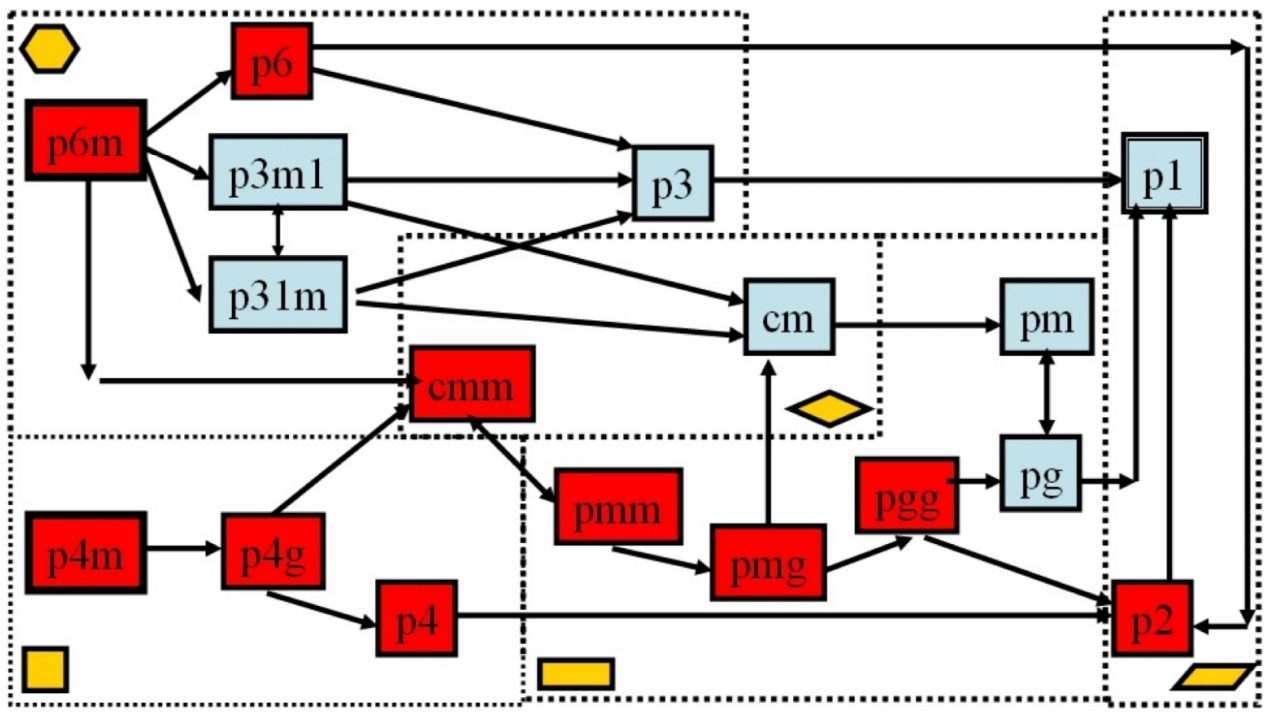
\includegraphics[width=0.9\columnwidth]{Yanxi_Graph}
\label{graph}
\caption{The subgroup relation graph}
\end{figure}

No interaction terms were considered, so the equation was simply: 

\[\mathrm{acc} \sim \mathrm{rot}+\mathrm{ref}+\mathrm{gref}+\mathrm{tile}+\mathrm{distance}+(1\mid \mathrm{subject})+(1 \mid \mathrm{task})\]

To be clear, accuracy (acc) in each record was 1 or 0. Rotation (rot), reflection (ref), glide reflection (gref), and tile shape (tile) were all either true or false based on whether the target image had the same value as the distracter image. The subject and the task were numeric based on their ID in the database. Please see Table~\ref{results} for a break-down of the results.

This shows that tile shape, glide reflection, and distance were all significant in determining accuracy. However, neither reflection or rotation are.

\begin{table}
\centering
\begin{tabular}{|l|ccc|}
\hline
& Estimate & Std. Error & t value \\ \hline
Rotation& 0.005650& 0.007742& 0.73 \\ \hline
Reflection& -0.004545& 0.005768& -0.79 \\ \hline
Glide Reflection& 0.06854& 0.005382& 3.13* \\ \hline
Tile& -0.030277& 0.006732& -3.87* \\ \hline 
Distance& 0.028984& 0.002781& 10.42* \\ \hline
\end{tabular}
\label{results}
\caption{Fixed Effects}
\end{table}